\documentclass{beamer}
 

\begin{document}


\begin{frame}{Baseline Coral-Fish Population Growth}
\begin{columns}[t]
\begin{column}[T]{8cm}
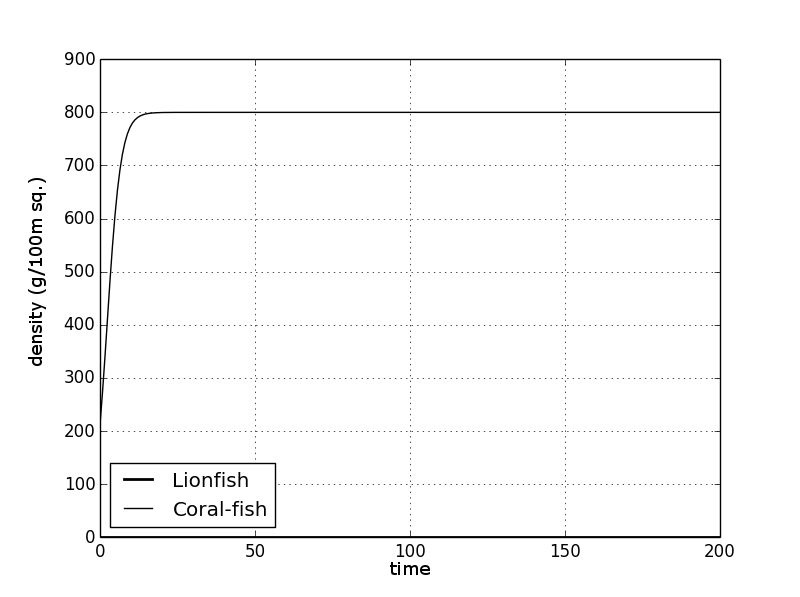
\includegraphics[height=7cm,width=8.5cm]{figure1.png}
\end{column}
\begin{column}[T]{3cm}

\begin{itemize}

\item C0 = 212

\item RC = .447

\item K = 800

\end{itemize}

\end{column}
\end{columns}
\end{frame}

\begin{frame}{Introducing Lionfish Population\\ at a Reduced Conversion Rate}
\begin{columns}[t]
\begin{column}[T]{8cm}
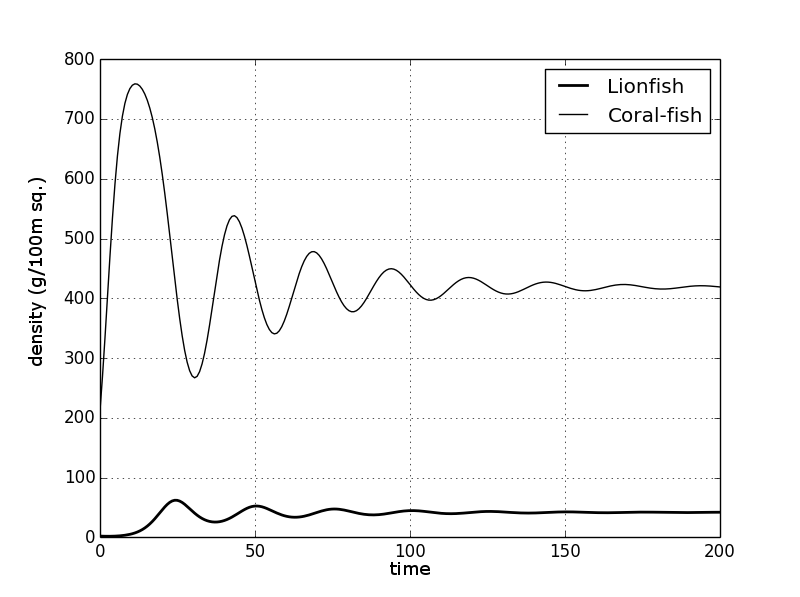
\includegraphics[height=7cm,width=8.5cm]{figure2.png}
\end{column}
\begin{column}[T]{3cm}
\begin{itemize}

\item $h_{CL}$ = 8.6/240

\item $b_{L}$ = .02

\item $d_{L}$ = .3


\end{itemize}
\end{column}
\end{columns}
\end{frame}

\begin{frame}{Half "Rule of ten" Conversion Rate}
\begin{columns}[t]
\begin{column}[T]{8cm}
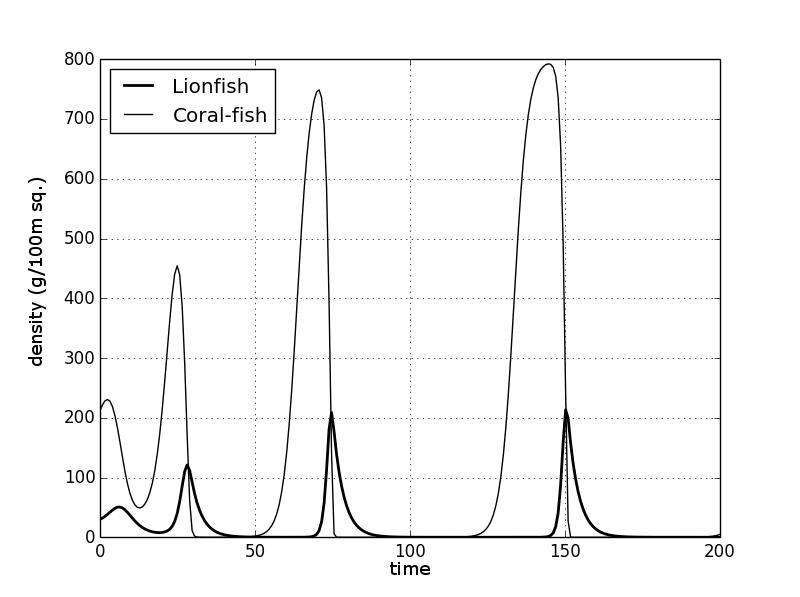
\includegraphics[height=7cm,width=8.5cm]{figure4.png}
\end{column}
\begin{column}[T]{3cm}
\begin{itemize}

\item $h_{CL}$ = 8.6/240

\item $b_{L}$ = .05

\item $d_{L}$ = .3


\end{itemize}
\end{column}
\end{columns}
\end{frame}

\begin{frame}{"Rule of ten"  Conversion Rate}
\begin{columns}[t]
\begin{column}[T]{8cm}
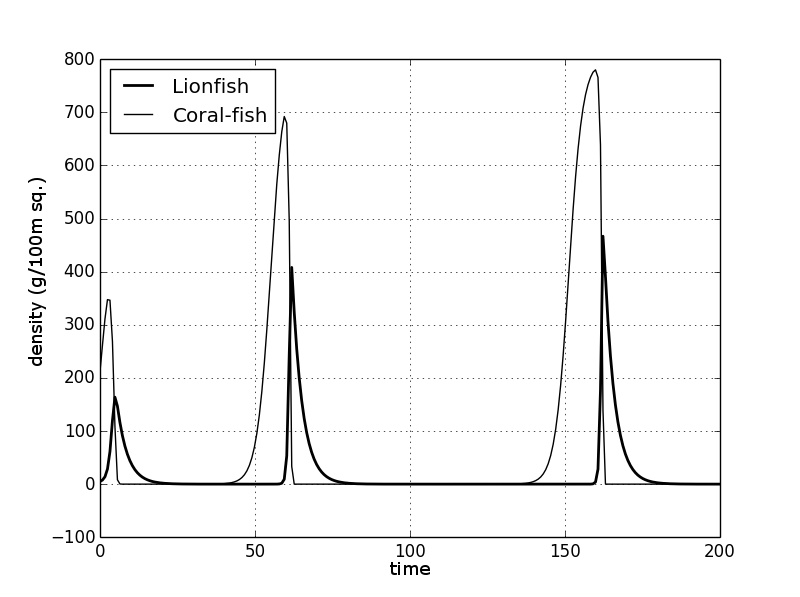
\includegraphics[height=7cm,width=8.5cm]{figure3.png}
\end{column}
\begin{column}[T]{3cm}
\begin{itemize}

\item $h_{CL}$ = 8.6/240

\item $b_{L}$ = .1

\item $d_{L}$ = .3


\end{itemize}
\end{column}
\end{columns}
\end{frame}


\begin{frame}{Introducing Grouper Harvesting}
\begin{columns}[t]
\begin{column}[T]{8cm}
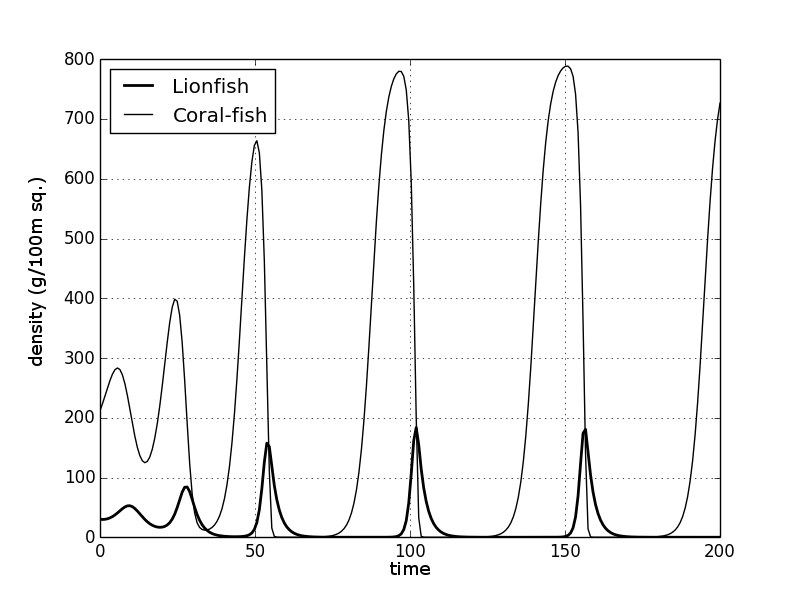
\includegraphics[height=7cm,width=8.5cm]{figure5.png}
\end{column}
\begin{column}[T]{3cm}
\begin{itemize}

\item $h_{LG}$ = 0.1



\end{itemize}
\end{column}
\end{columns}
\end{frame}

\begin{frame}{Increasing Grouper Harvest}
\begin{columns}[t]
\begin{column}[T]{8cm}
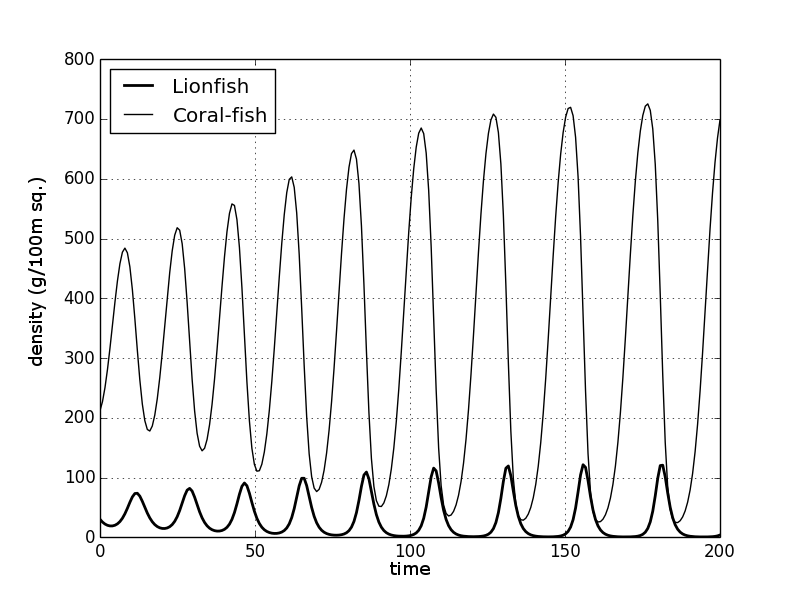
\includegraphics[height=7cm,width=8.5cm]{figure6.png}
\end{column}
\begin{column}[T]{3cm}
\begin{itemize}

\item $h_{LG}$ = 0.3



\end{itemize}
\end{column}
\end{columns}
\end{frame}

\begin{frame}{Extended Time}
\begin{columns}[t]
\begin{column}[T]{8cm}
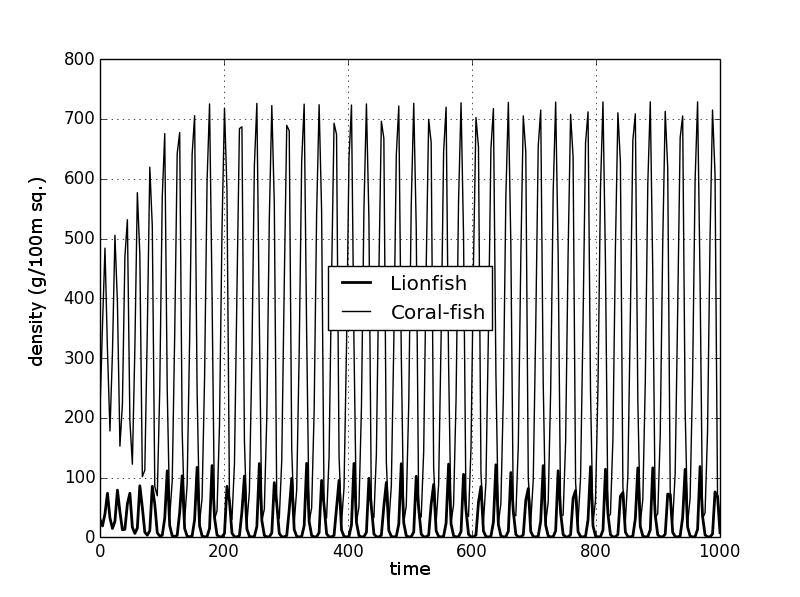
\includegraphics[height=7cm,width=8.5cm]{figure6b.png}
\end{column}
\begin{column}[T]{3cm}
\begin{itemize}

\item $h_{LG}$ = 0.3



\end{itemize}
\end{column}
\end{columns}
\end{frame}

\begin{frame}{Significant Increase in Grouper Harvest}
\begin{columns}[t]
\begin{column}[T]{8cm}
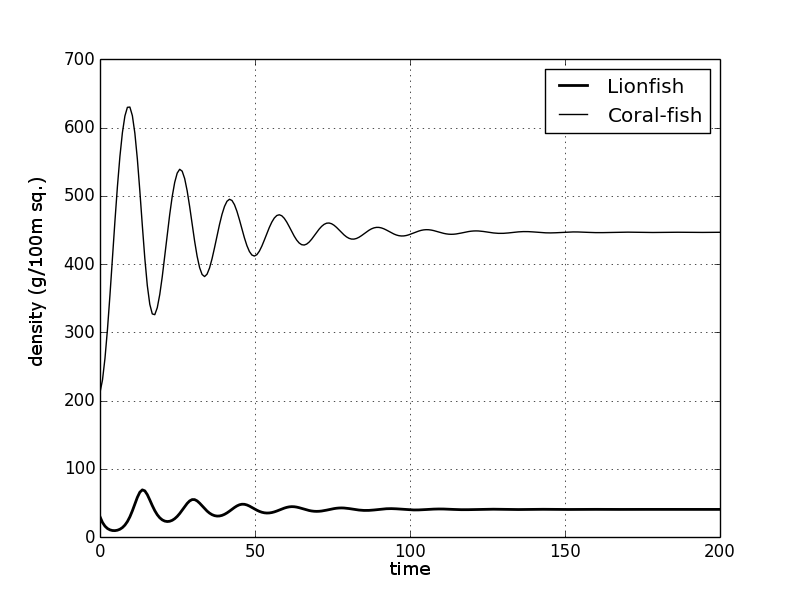
\includegraphics[height=7cm,width=8.5cm]{figure7.png}
\end{column}
\begin{column}[T]{3cm}
\begin{itemize}

\item $h_{LG}$ = 0.5



\end{itemize}
\end{column}
\end{columns}
\end{frame}


\begin{frame}{Decreasing Grouper Harvest\\ to Find Threshold}
\begin{columns}[t]
\begin{column}[T]{8cm}
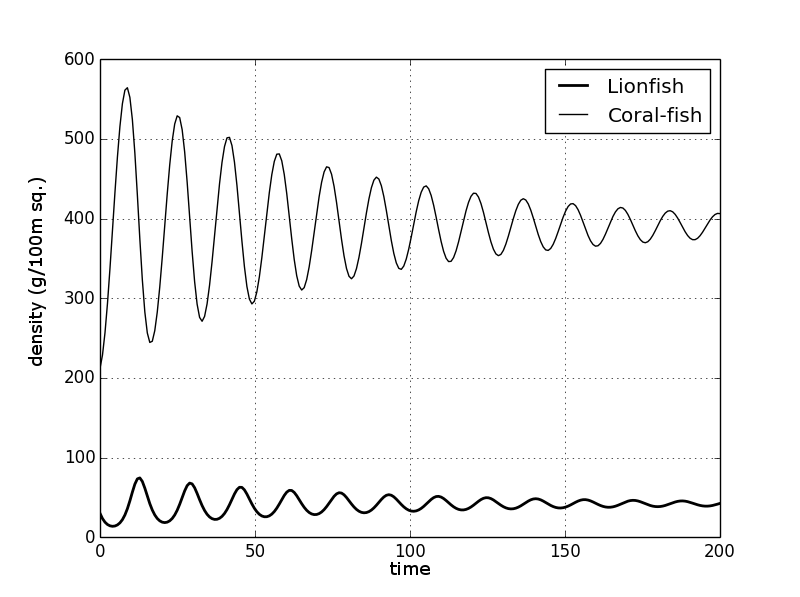
\includegraphics[height=7cm,width=8.5cm]{figure9.png}
\end{column}
\begin{column}[T]{3cm}
\begin{itemize}

\item $h_{LG}$ = 0.40



\end{itemize}
\end{column}
\end{columns}
\end{frame}

\begin{frame}
\begin{columns}[t]
\begin{column}[T]{8cm}
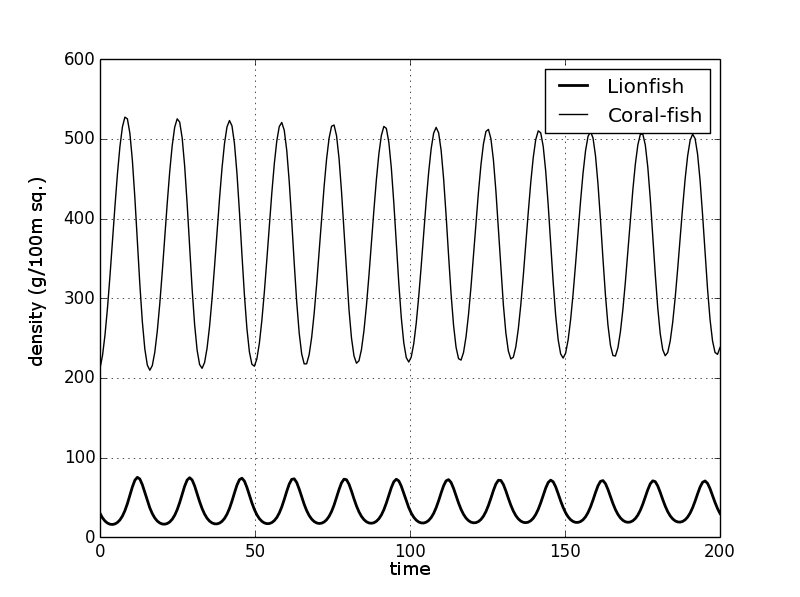
\includegraphics[height=7cm,width=8.5cm]{figure11.png}
\end{column}
\begin{column}[T]{3cm}
\begin{itemize}

\item $h_{LG}$ = 0.3525



\end{itemize}
\end{column}
\end{columns}
\end{frame}

\begin{frame}
\begin{columns}[t]
\begin{column}[T]{8cm}
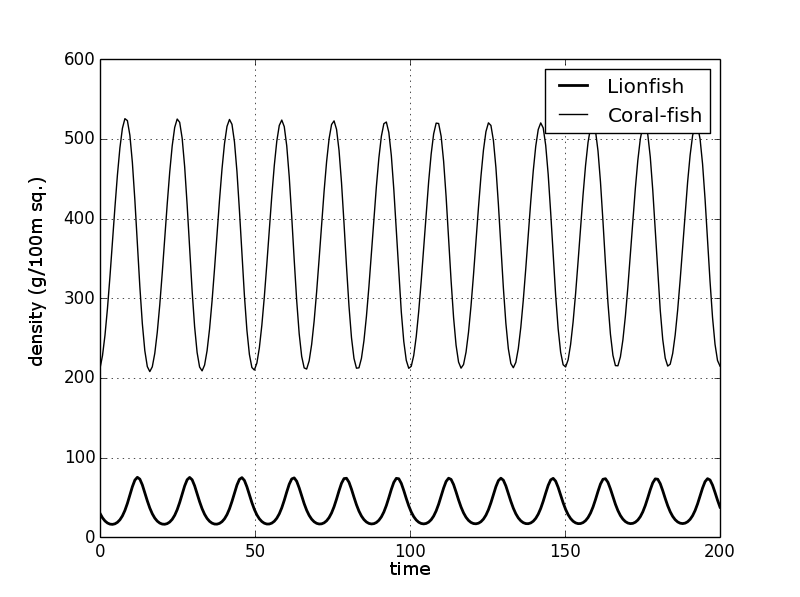
\includegraphics[height=7cm,width=8.5cm]{figure10.png}
\end{column}
\begin{column}[T]{3cm}
\begin{itemize}

\item $h_{LG}$ = 0.349



\end{itemize}
\end{column}
\end{columns}
\end{frame}


\begin{frame}
\begin{columns}[t]
\begin{column}[T]{8cm}
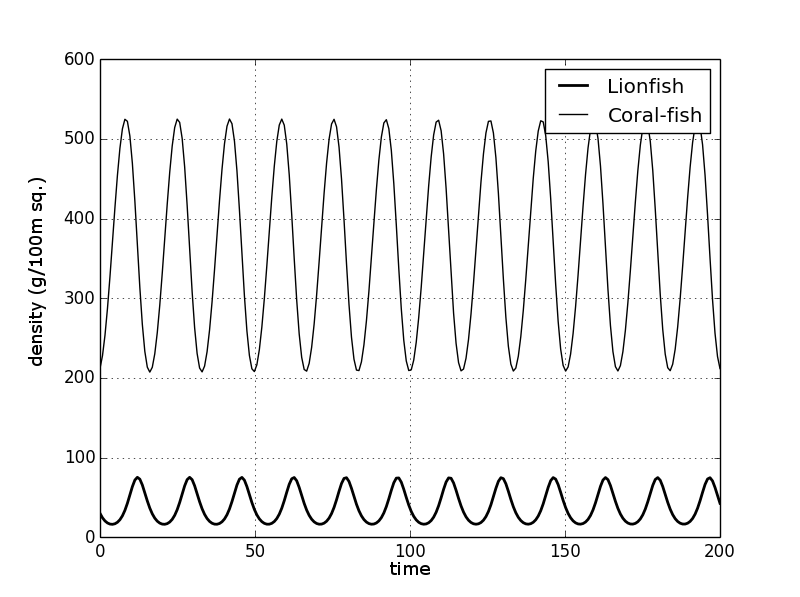
\includegraphics[height=7cm,width=8.5cm]{figure12.png}
\end{column}
\begin{column}[T]{3cm}
\begin{itemize}

\item $h_{LG}$ = 0.35



\end{itemize}
\end{column}
\end{columns}
\end{frame}

\begin{frame}
\begin{columns}[t]
\begin{column}[T]{8cm}
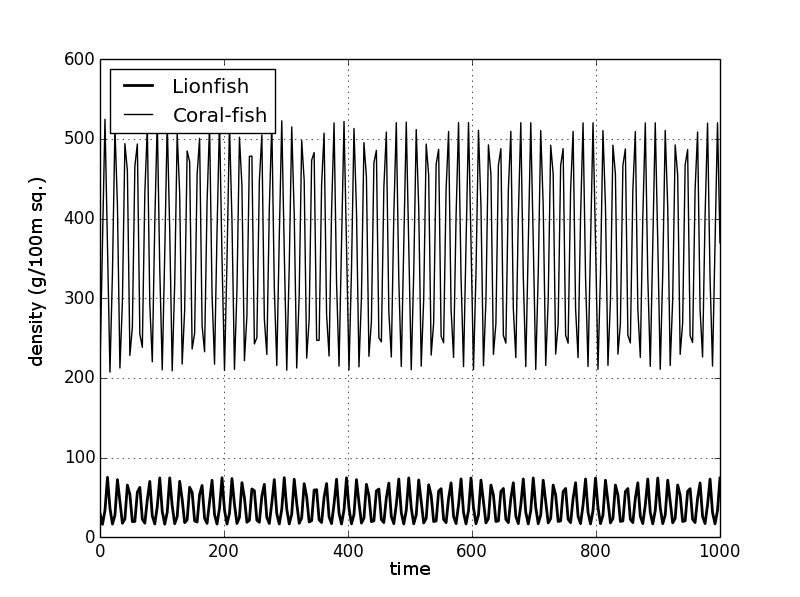
\includegraphics[height=7cm,width=8.5cm]{figure12b.png}
\end{column}
\begin{column}[T]{3cm}
\begin{itemize}

\item $h_{LG}$ = 0.35



\end{itemize}
\end{column}
\end{columns}
\end{frame}





\end{document}